\documentclass[10pt]{article}
\author{Lawrence Liu}
\usepackage{subcaption}
\usepackage{graphicx}
\usepackage{amsmath}
\usepackage{pdfpages}
\newcommand{\Laplace}{\mathscr{L}}
\setlength{\parskip}{\baselineskip}%
\setlength{\parindent}{0pt}%
\usepackage{xcolor}
\usepackage{listings}
\definecolor{backcolour}{rgb}{0.95,0.95,0.92}
\usepackage{amssymb}
\usepackage{empheq}

\newcommand*\widefbox[1]{\fbox{\hspace{2em}#1\hspace{2em}}}
\lstdefinestyle{mystyle}{
    backgroundcolor=\color{backcolour}}
\lstset{style=mystyle}

\usepackage{geometry}
\geometry{a4paper,margin=0.25in}
\begin{document}
\underline{\textbf{Signals}}\\
A discrete time signal can be described as a mathematical function $x[n]$ where $n$ is the index of the sample.
Or as an Array/List of the significant samples, with any sample not listed being 0. 
Or by plotting. We can modify a signal by multiplying it by something or adding something to it. We can also
modify the signal by time shifting it: ie $X(t-3)$ will delay the signal by shifting it to the right, and $X(t+3)$ will
advance the signal by shifting it to the left. Likewise we can multiply the signal by a constant $c>1$ will effectively
"downsample" the signal, and multiplying it by $c<1$ will "upsample" the signal. Likewise we can time reverse the signal. \\
\underline{\textbf{Delta and Unit Step Signals}}\\
We define the \textbf{delta signal} as $\boxed{\delta[n]=\begin{cases}1 & n=0\\0 & n\neq 0\end{cases}}$. From this we have the following sampling
property: $\boxed{x[n]\cdot\delta[n-k]=x[k]\delta[n-k]}$. From this delta signal we can define the \textbf{unit step} signal 
$\boxed{u[n]=\sum_{k=0}^{\infty}\delta[n-k]=\begin{cases}1 & n\geq 0\\0 & n<0\end{cases}}$.\\
\underline{\textbf{Periodicity}}\\
A signal is periodic if it can be written as $x[n]=x[n+N]$ for some integer $N$ and all $n$. A signal's fundamental period 
is the smallest integer $N$ such that $x[n]=x[n+N]$ for all $n$.\\
\underline{\textbf{Even and Odd Signals}}\\
A signal is even if $x[n]=x[-n]$. A signal is odd if $x[n]=-x[-n]$. We can decompose any singal into its even and odd parts
with the even part $x_e[n]=\frac{1}{2}(x[n]+x[-n])$ and the odd part $x_o[n]=\frac{1}{2}(x[n]-x[-n])$.\\
\underline{\textbf{Energy and Power Signals}}\\
We define the energy of a signal as $\boxed{E=\sum_{n=-\infty}^{\infty}|x[n]|^2}$. We define the power of a signal as $
\boxed{P=\lim_{m\to\infty}\frac{1}{2m+1}\sum_{n=-\infty}^{M}|x[n]|^2}$. If the signal is periodic, this can be 
simplified to $\boxed{P=\frac{1}{N}\sum_{n=0}^{N-1}|x[n]|^2}$. We call a signal a \textbf{energy signal} if its energy is finite, and a \textbf{power signal} if its power is finite.
A power signal will have infinite energy.\\
\underline{\textbf{System Properties}}\\
A system is \textbf{linear} if given the outputs $y_1[n]$, and $y_2[n]$ of two inputs $x_1[n]$ and $x_2[n]$ respectively, 
then the output of the input $x_3=\alpha x_1[n]+\beta x_2[n]$ the output is $y_3[n]=\alpha y_1[n]+\beta y_2[n]$. 
A system is \textbf{time invariant} if given the output $y[n]$ of an input $x[n]$, then the output of the input $x[n-k]$ is $y[n-k]$. A system is \textbf{causal} if the output of an input $x[n]$ is only dependent on the input $x[n]$ and not $x[n-k]$ for $k<0$. 
A system is \textbf{stable} if the output of an input $x[n]<\alpha<\infty$ for all $n$, the output $y[n]<\beta<\infty$ for all $n$. A
system is \textbf{relaxed} if the output for an input $x[n]\to0$ for $n\to\infty$, then $y[n]\to0$ for $n\to\infty$.\\
\underline{\textbf{Convolution}}\\
We define the convolution of two signals $x[n]$ and $h[n]$ as $\boxed{y[n]=x[n]*h[n]=\sum_{k=-\infty}^{\infty}x[k]h[n-k]}$. A shortcut on how to do 
convolution is shown below:\\
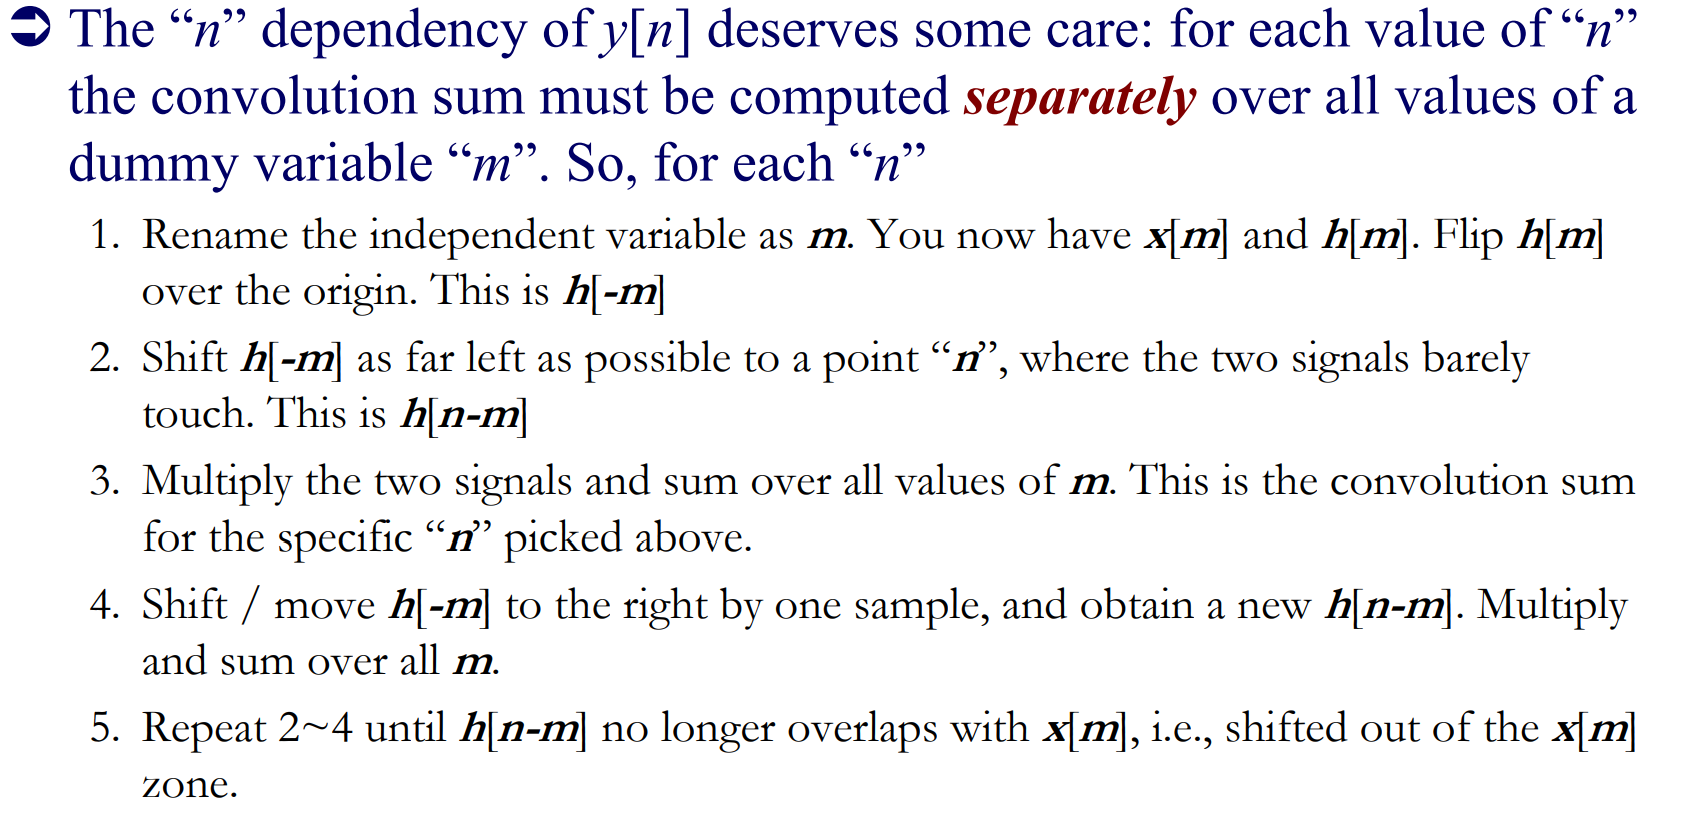
\includegraphics[width=0.5\textwidth]{convolution.png}\\
We have that if given two signals $x_1[n]$ and $x_2[n]$ that start at $n_1$ and $n_2$ respectively and have lengths of 
$L_1$ and $L_2$ respectively, then the convolution of the two signals will have nonzeros values for $n_1+n_2\leq n\leq n_1+n_2+L_1+L_2$, and thus
the convolution will have $L_1+L_2+1$ nonzero values. \\
\underline{\textbf{Discrete Time Fourier Transform}}\\
If a signal is periodic with period $N$, then we have that we can represnt it as a discrete fourier series, $\boxed{x[n]=\frac{1}{N}\sum_{k=0}^{N-1}c_ke^{j\frac{2\pi}{N}kn}}$. Where
$c_k$ is derived from $\boxed{c_k=\sum_{n=0}^{N-1}x[n]e^{-j\frac{2\pi}{N}kn}}$.


\end{document}
